\chapter{Marco Metodológico}
\section{Proceso de Obtención de Datos}
El proceso de obtención de datos para el entrenamiento de los algoritmos se realizó por medio de entrevistas a distintos individuos. La población objetivo para estas entrevistas se delimitó a estudiantes y colaboradores de la Universidad del Valle de Guatemala. El proceso de extracción de información se realizó mediante pruebas dentro de estas entrevistas, a las cuales los individuos de estudio se ofrecían voluntariamente para tomarlas mediante una solicitud con un formulario electrónico en línea. Estas pruebas fueron realizadas en un ambiente controlado dentro de las instalaciones de las Clínicas de Psicología de la Universidad del valle de Guatemala, durante los meses de marzo y abril del año 2018. 

Estas entrevistas se realizaron a cincuenta y seis (56) sujetos pertenecientes al grupo de estudio objetivo. Un estudio con un número de participantes mayor a veintidós puede aportar mejores resultados (Davatzikos et al., 2005). Cada participante proporcionó algunos datos personales para determinar datos  sobre la población en la cual se realizó el experimento. Estos datos incluyen género, edad, lateralidad, escolaridad, grupo étnico, estado civil, sector de población universitaria a la que pertenecen, empleo y acompañamiento psicológico. De igual manera, se realizaron pruebas psicometrícas a los individuos de estudio durante el proceso de entrevista, acompañados por estudiantes de la facultad de Psicología. Además que estos datos permiten determinar posibles variables relacionadas con el engaño, estos también pueden ser útiles para las personas que deseen utilizar el conjunto de datos para otros estudios o para continuar el presente trabajo.

Durante las entrevistas realizadas, se pidió a los participantes responder a una serie de preguntas seleccionadas que un moderador les realizaría. Estas preguntas se realizaron durante dos rondas. En la primera ronda, se solicitó al sujeto que respondiera a las preguntas diciendo la verdad. En la segunda ronda, se realizaron las mismas preguntas, pero se solicitó al sujeto que respondiera con falacias. Durante estas rondas de preguntas, la extracción de la información se realizó por medio de distintos instrumentos de medición relacionados a los módulos del proyecto. Las entrevistas fueron grabadas con vídeo y audio, además de utilizar los instrumentos de medición de ondas electroencefalográficas.

La obtención de datos de la actividad electroencefalográfica de los sujetos se realzó mediante el uso de un casco \textit{Emotiv EPOC} y su conexión a un ordenador con el panel de control \textit{Emotiv Xavier}. El uso del dispositivo para la extracción de la información se hizo empleando el proyecto \textit{EMOTRIX}. El proyecto Emotrix es una plataforma que permitirá el estudio, identificación y manipulación de emociones humanas. La plataforma se podrá utilizar para fines educativos, médicos o recreacionales, entre otros. A la fecha, existen distintos dispositivos que permiten imitar inteligencia emocional, los cuales tienen precios elevados. Es por esto por lo que la plataforma tiene un enfoque de código libre para permitir el desarrollo de forma abierta y evitar cualquier tipo de restricciones a los usuarios. El ámbito al que pertenece el proyecto es a la interacción humano – computador (HCI). Este proyecto ha sido desarrollado desde 2016 por estudiantes de la Universidad del Valle de Guatemala.

\section{Análisis Exploratorio de los Datos}
Se obtuvieron una serie de variables de distintos tipos procedentes de las pruebas realizadas en las entrevistas. Se obtuvieron quince (15) variables procedentes de Emotiv EPOC, referentes a los canales de lectura del mismo. Se obtuvieron doce (12) variables descriptivas de los individuos entrevistados y de sus pruebas psicométricas asociadas. Estas últimas son género, edad, lateralidad, escolaridad, grupo étnico, estado civil, prueba l1 ,prueba l2, sector de la población de la universidad a la que pertenecen, empleo, acompañamiento psicológico y tipo de acompañamiento psicológico. Para un total de veintisiete variables. De las variables electroencefalográficas, se tomó únicamente las que procedían de los transmisores ubicados en los lóbulos frontales. Esto se debe a que se sugiere que las emociones relacionadas con el engaño se encuentran en esta parte del cerebro humano (Belmonte C., 2007). Por lo que se trabajaron ocho (8) variables de este tipo, referente a los canales AF3, AF4, F3, F4, F7, F8, FC5 y FC6. 

\begin{figure}
    \centering
    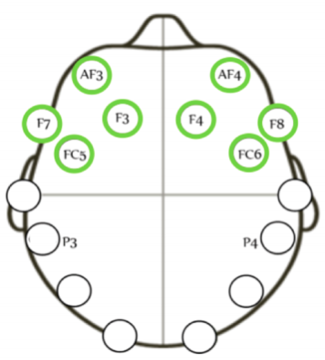
\includegraphics[scale=1]{figuras/Imagen2.png}
    \caption{Electrodos EPOC a considerar para la selección de variables.}
    \label{fig:my_label}
\end{figure}




\section{Construcción del Conjunto de Datos de Entrenamiento}
\section{Desarrollo del Modelo de Clasificación}
\section{Desarrollo del la Interfaz de Respuesta}



\chapter{Resultados}
A estas variables se les realizó un análisis de regresión logística y de árboles de decisión para obtener las más significativas para el estudio. Estos análisis fueron realizados empleando el lenguaje de programación R y el software \textit{RStudio}. Los resultados de estos análisis se muestran a continuación:

\begin{figure}
    \centering
    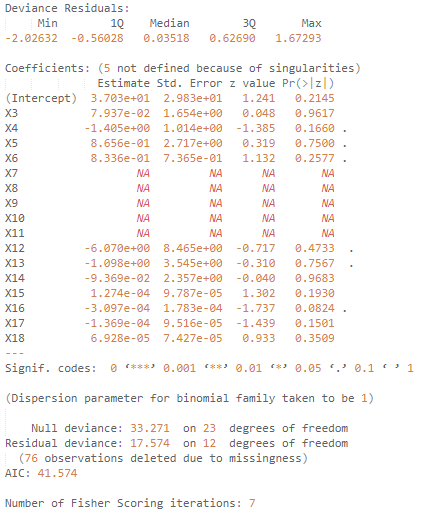
\includegraphics[scale=1]{figuras/Capture4.PNG}
    \caption{Resultados del análisis de regresión logística.}
    \label{fig:my_label}
\end{figure}

\begin{figure}
    \centering
    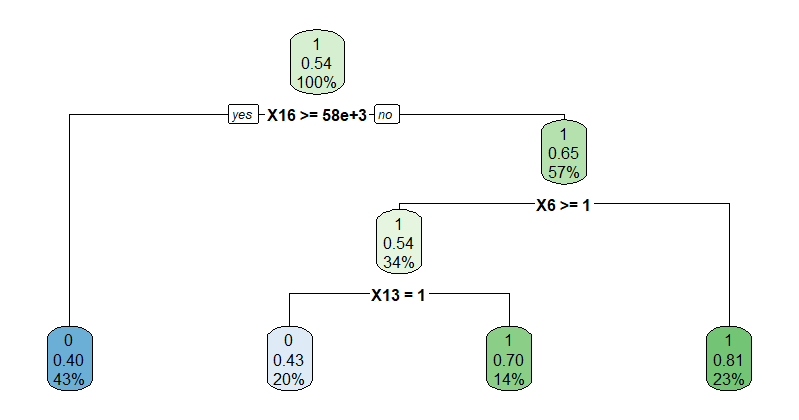
\includegraphics[scale=0.75]{figuras/Rplot1.png}
    \caption{Resultados del análisis de árbol de decisión.}
    \label{fig:my_label}
\end{figure}

\begin{figure}
    \centering
    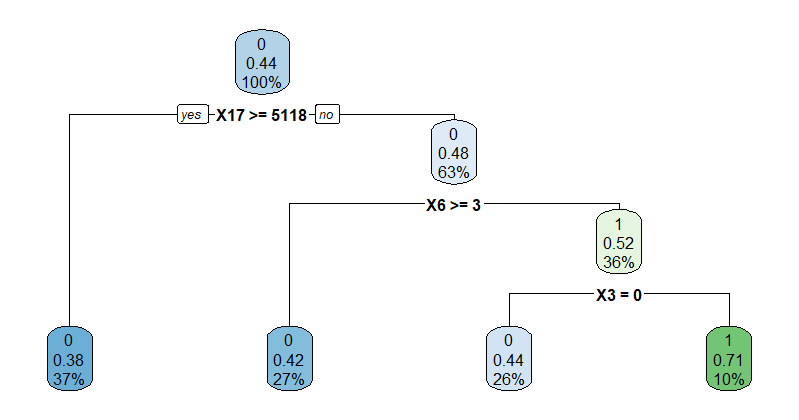
\includegraphics[scale=0.75]{figuras/Rplot2.png}
    \caption{Resultados del análisis de árbol de decisión.}
    \label{fig:my_label}
\end{figure}

A partir de estos resultados, se obtuvieron las variables más significativas para poder entrenar los algoritmos de aprendizaje de máquina. Estas son un total de catorce (14) variables, ocho (8) de electroencefalograma y seis (6) de variables descriptivas. Estas variables descriptivas son: edad, lateralidad, escolaridad, empleo y acompañamiento psicológico. 









\begin{center}
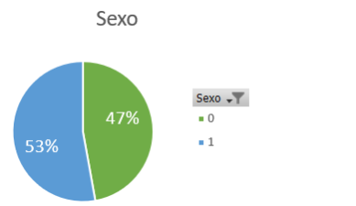
\includegraphics[height=1.15in]{figuras/Imagen11.png}
\end{center}

\begin{center}
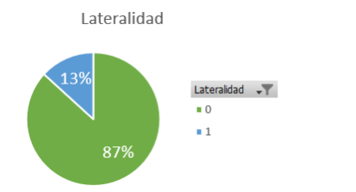
\includegraphics[height=1.15in]{figuras/Imagen12.png}
\end{center}

\begin{center}
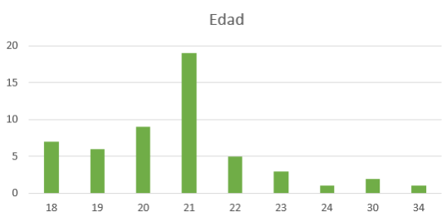
\includegraphics[height=1.15in]{figuras/Imagen13.png}
\end{center}

\begin{center}
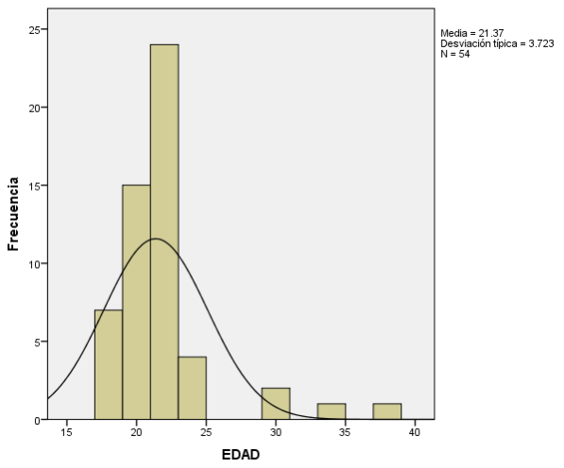
\includegraphics[height=1.15in]{figuras/Imagen14.png}
\end{center}

\begin{center}
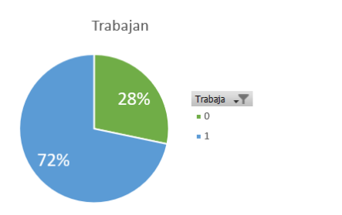
\includegraphics[height=1.15in]{figuras/Imagen15.png}
\end{center}

\begin{center}
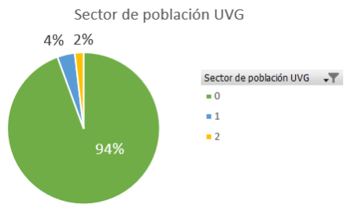
\includegraphics[height=1.15in]{figuras/Imagen16.png}
\end{center}

\begin{center}
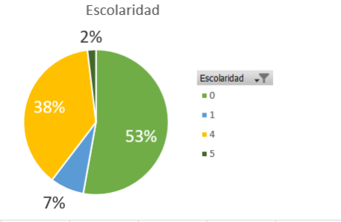
\includegraphics[height=1.15in]{figuras/Imagen17.png}
\end{center}

\begin{center}
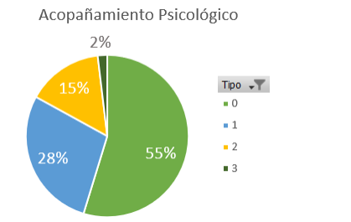
\includegraphics[height=1.15in]{figuras/Imagen18.png}
\end{center}

\begin{center}
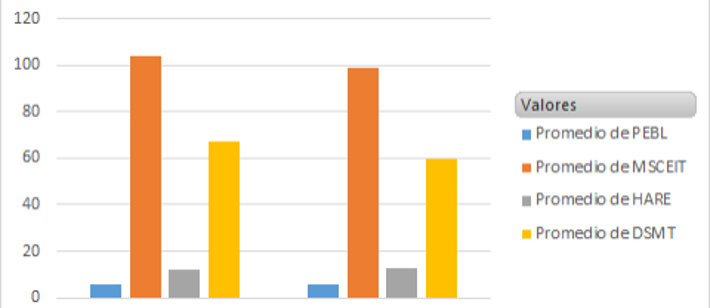
\includegraphics[height=1.15in]{figuras/Imagen19.png}
\end{center}



\begin{center}
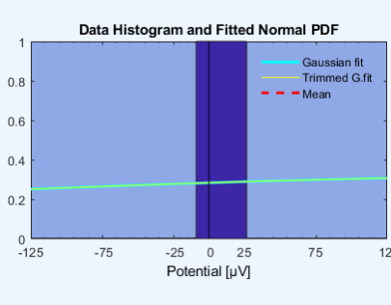
\includegraphics[height=2.35in]{figuras/Imagen7.png}
\end{center}

\begin{center}
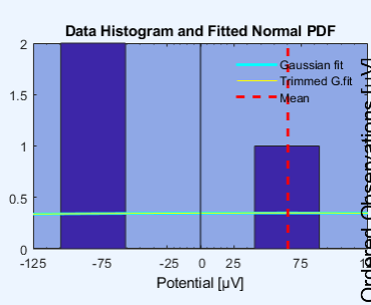
\includegraphics[height=2.35in]{figuras/Imagen8.png}
\end{center}

\begin{center}
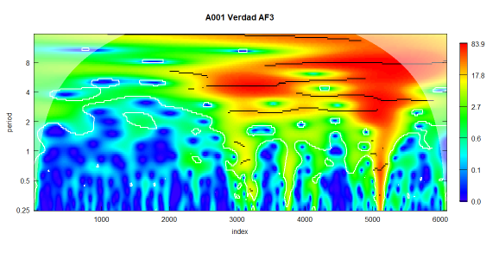
\includegraphics[height=3.0in]{figuras/Imagen9.png}
\end{center}

\begin{center}
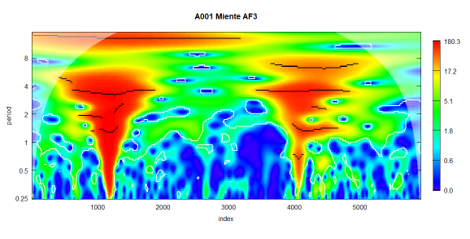
\includegraphics[height=3.0in]{figuras/Imagen10.png}
\end{center}



\begin{center}
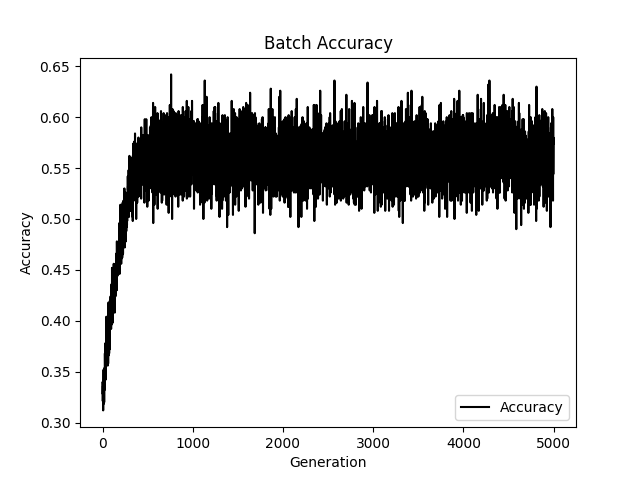
\includegraphics[height=3.0in]{figuras/Figure_1.png}
\end{center}

\begin{center}
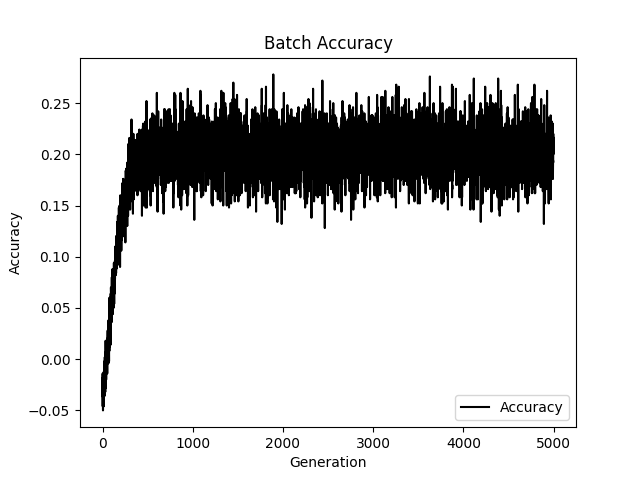
\includegraphics[height=3.0in]{figuras/Figure_2.png}
\end{center}

\begin{center}
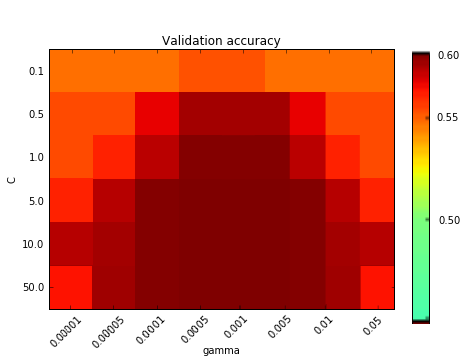
\includegraphics[height=3.0in]{figuras/58e171451b12ce00012bd71d.png}
\end{center}

\begin{center}
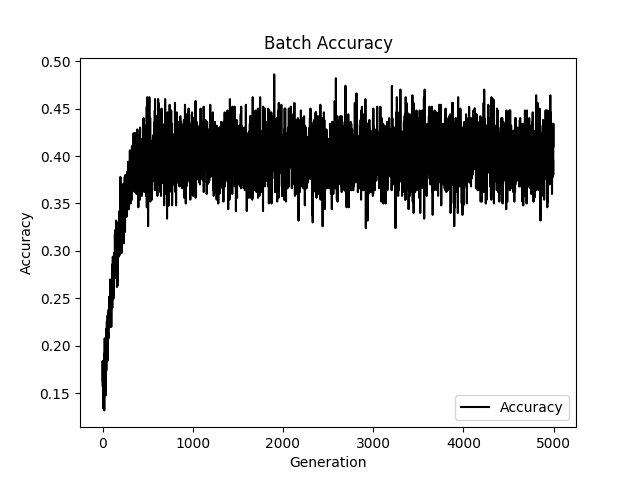
\includegraphics[height=3.0in]{figuras/Figure_3.png}
\end{center}

\begin{center}
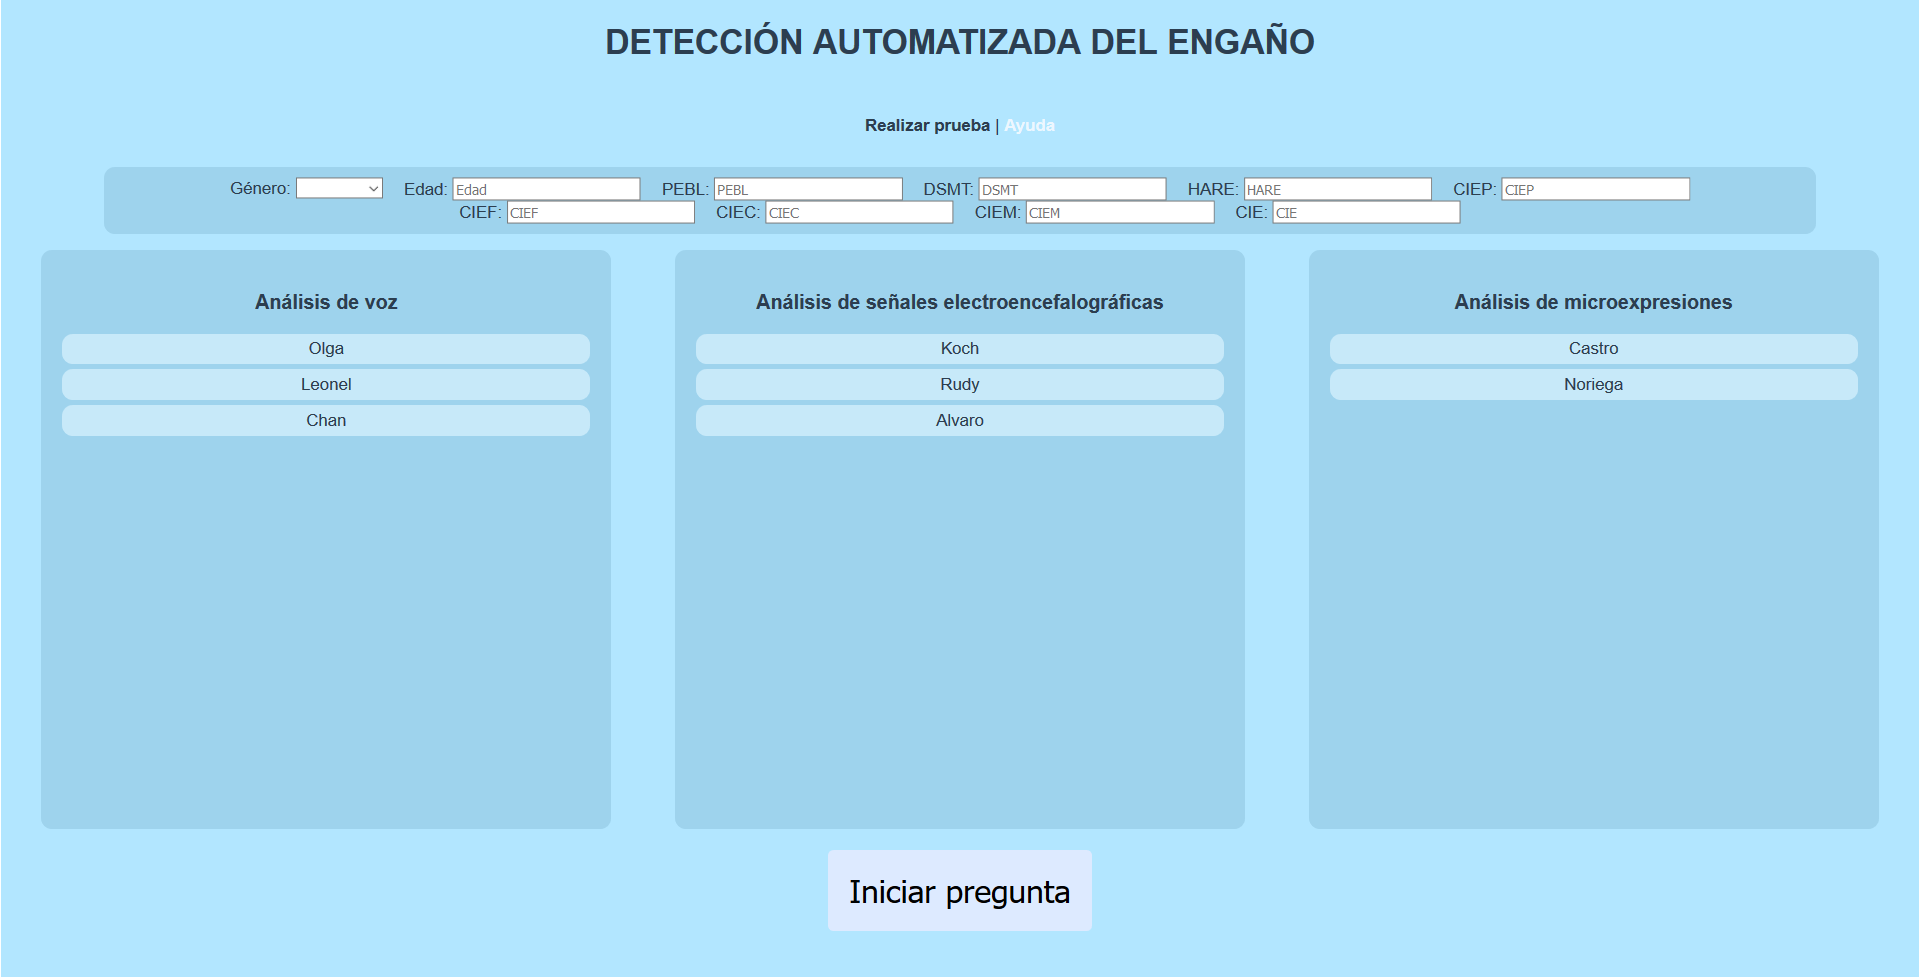
\includegraphics[height=3.15in]{figuras/Imagen20.PNG}
\end{center}



\chapter{Análisis de Resultados}





%\section{Dinámica de cuerpos rígidos}
%\section{Restricciones}
%\subsection{Mecanismos de lazo cerrado}
%\subsubsection{Mecanismo de cuatro barras}
%\chapter{Control del sistema mecánico}
%\section{La ecuación del manipulador}